\chapter{Approach}

\label{Chapter3}

\lhead{Chapter 3. \emph{Approach}}

\section{System overview} % (fold)
\label{approach:sec:system_overview}

The proposed system is constructed around the data flowing through it. This chapter describes each part of the system outlined in figure~\ref{fig:system-architecture}.

\begin{figure}[b]
  \centering
    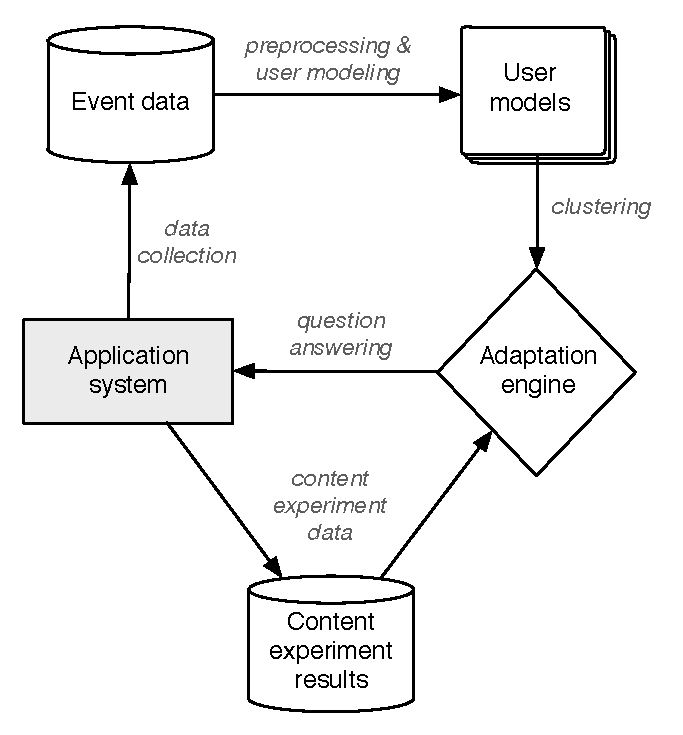
\includegraphics[width=0.6\textwidth]{Figures/system-architecture}
    \caption{Overview of the system architecture.}
    \label{fig:system-architecture}
\end{figure}

The system begins by taking the data stepwise through an ingestion pipeline, importing, filtering, and cleaning it. The steps of the ingestion pipeline are discussed in section~\ref{approach:sec:data_ingestion_and_preprocessing}, before moving on to the user modeling component in section~\ref{approach:sec:user_modeling}.

Once user models are in place, the system identifies user segments. These are stored in a database for future use. This process is discussed in more detail in section~\ref{approach:clustering}.

Apart from clusters, the adaptation component requires content experiment results to predict how users will respond to application variations. This is discussed in section~\ref{approach:sec:feature_experiments}.

The components come together in the adaptation component, discussed in section~\ref{approach:sec:adaptation_component}, whose job it is to answer questions about users, effectively completing the feedback cycle back to the application.

% section system_overview (end)

\section{Data ingestion and preprocessing} % (fold)
\label{approach:sec:data_ingestion_and_preprocessing}

Before the interesting parts of the system can start doing their work, the data needs to be transformed from \emph{a series of chronological raw events} to \emph{a set of user models}.

The amount of data can be arbitrarily sizable, and will grow linearly with user activity. The system architecture has been designed to be able to cope with this; its functional and data-driven nature should be easily adaptable to hugely scalable programming paradigms like MapReduce.

\begin{figure}[h]
  \centering
    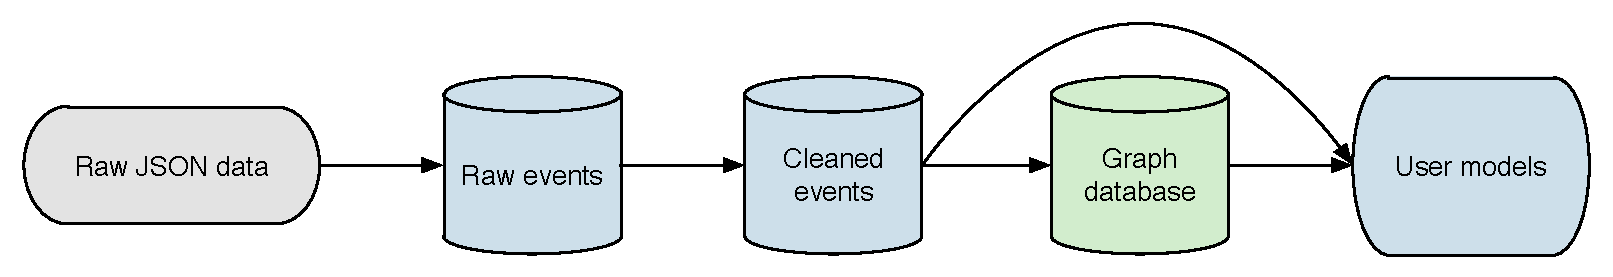
\includegraphics[width=\textwidth]{Figures/ingestion-pipeline}
  \caption{The ingestion pipeline broken into 4 steps. The color of each node indicates means of storage: \emph{Blue} indicates a RDBMS, \emph{green} indicates a graph database, whereas \emph{gray} is used to indicate flat file storage.}
  \label{fig:ingestion-pipeline}
\end{figure}

\subsection{Generating the raw data}
\label{approach:sub:generating_data}

The system input is a chronological series of raw events sent from the production system. The events are instrumented via an external analysis service called KISSmetrics\footnote{\url{https://www.kissmetrics.com/}} -- a user analysis system designed around tracking individual users' behavior.

The application logs an event by calling the KISSmetrics REST API. The following data is in each instrumentation call:

\begin{enumerate}
  \item person identifier
  \item event name
  \item user properties (optional)
\end{enumerate}

The consistency of the personal identifier has already been discussed extensively in the introductory chapters, especially section~\ref{intro:sub:anonymity_privacy}, but a short technical introduction to the actual production system is in order.

To enable effective utilization of the KISSmetrics instrumentation functionality, they supply a client library for the purpose. This client library handles a few central things for us:

\begin{enumerate}
  \item Person identity storage and loading over subsequent page loads.
  \item The low-level instrumentation of events.
  \item Simple A/B testing facilities.
\end{enumerate}

When the KISSmetrics client library is loaded, the person identity is automatically either retrieved from the browser cookies, or generated. The identity of a person is a unique randomly generated string, which serves no other purpose than to track the identity of the browser over time.

Whenever something ``interesting'' happens, an event is sent to the KISSmetrics instrumentation service. An ``interesting'' event is typically anything that tells us about how the users use the service, both in terms of general activity and in terms of feature adoption. Every event is tagged with the person identity, as well as an event name and a timestamp.

The KISSmetrics service provides several analytical tools to dig into this data, thereamongst funnel reports (example in figure~\ref{fig:funnel-report}) and cohort reports.

\begin{figure}[h]
  \centering
    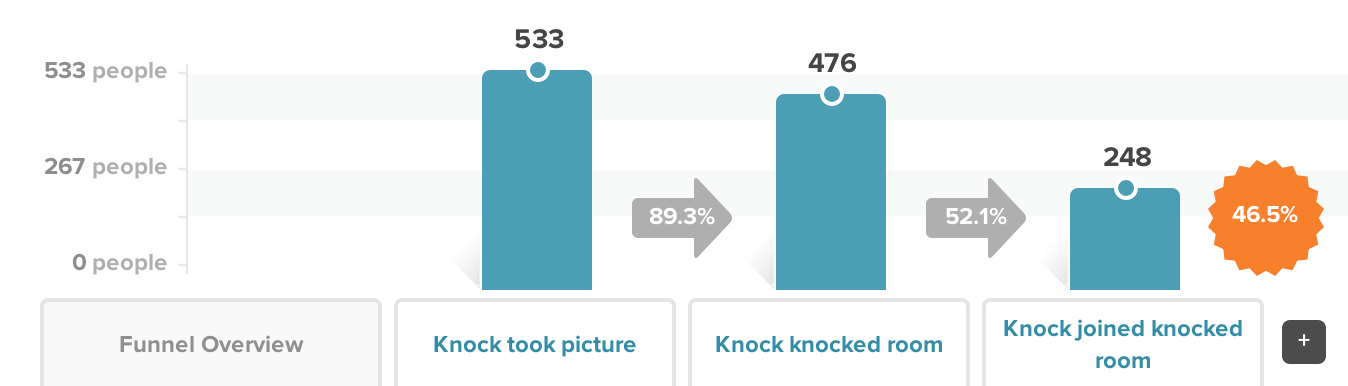
\includegraphics[width=\textwidth]{Figures/screenshots/km/funnel-example}
    \caption{Example of a simple funnel report.}
    \label{fig:funnel-report}
\end{figure}

% \begin{figure}[h]
%   \centering
%     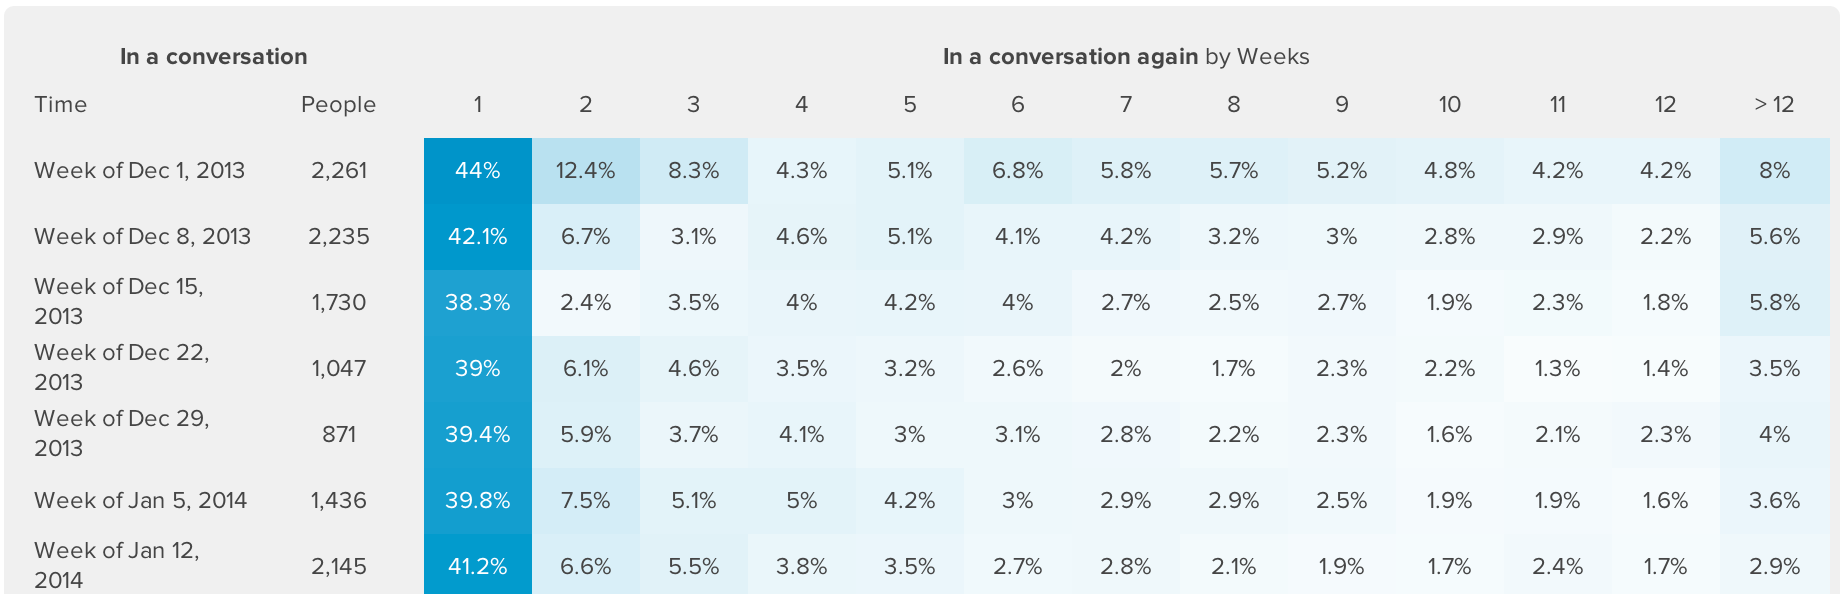
\includegraphics[width=\textwidth]{Figures/screenshots/km/cohort-example}
%     \caption{Example of a cohort report.}
%     \label{fig:cohort-report}
% \end{figure}

\subsection{Cleaning the data}
\label{approach:sec:cleaning_data}

KISSmetrics has the ability to export raw event data to data files. This can be used to power completely customized analyses, as will be needed for our particular task.

After the raw data has been aquired, it will need to be cleaned. This is a simple process of churning through each line of each unprocessed data file, parsing and splitting its contents into appropriate data fields, and inserting it into databases.\footnote{To facilitate the compilation of network-related user model features, conversation data was loaded into a graph database to enable querying of network structures.}

% section data_ingestion_and_preprocessing (end)

\section{User modeling} % (fold)
\label{approach:sec:user_modeling}

To find clusters of users, we first and foremost need to quantify them. More specifically, we want to represent each user as a numerical feature vector.

\subsection{Feature selection}
\label{approach:sec:feature_selection}

Given the types of events being collected, we landed on compiling the following features:

\begin{enumerate}
  \item First degree conversation partners
  \item Second degree conversation partners
  \item Inviter
  \item Invitee
  \item Conversations
  \item Rooms used
  \item Rooms claimed
  \item Roomnames generated
  \item Chat message sent
\end{enumerate}

To generate user models, the stream of event data were mapped to their associated users for aggregation. That is, the transformation in this step started with data in the form of \eqref{pre_user_model}.

\begin{equation}
  \langle \text{event}, \text{timestamp}, \text{person}, \text{metadata} \rangle
  \label{pre_user_model}
\end{equation}

And ended with data in the form of~\eqref{post_user_model}, where \emph{value} contains the aggregated value.

\begin{equation}
  \langle \text{person}, \text{feature}, \text{value} \rangle
  \label{post_user_model}
\end{equation}

\section{Clustering the users}
\label{approach:clustering}

We assume the following hypothesis holds, as a basis for the clustering approach to the user adaptation problem:

\begin{hypothesis}
The more similarly two people use a service, the more likely they are to respond similarly to it changing.
\end{hypothesis}

Thus, we want to segment the users in the following way: users in each segment should be as similar as possible, and as dissimilar those in other segments as possible. This scheme fits well with the two criterias for selecting an optimal clustering scheme, as described by Berry and Linoff~\cite{Berry1997}.

@TODO: Remember the bias introduced in section~\ref{survey:sub:generality}.

\subsection{Choice of algorithms}
\label{approach:sec:clustering_algorithms}

Three algorithms were implemented and experimented with: DBSCAN, mean-shift, and k-means. Of these, the k-means clearly proved itself as the most effective one, and as it also managed to produce adequate and meaningful results, it was chosen as the principal algorithm.

\subsubsection{The k-means clustering algorithm}
\label{subs:kmeans}

The k-means clustering algorithm takes as input a preset number of clusters, $k$, a similarity measure function, and a set of data vectors. Initially, it randomly chooses $k$ data vectors as centroids as a starting point for the process, before repeatedly performing a two-pass operation adjusting the centroids until convergence.

Section~\ref{code:kmeans} shows a simple python-esque implementation of the k-means algorithm.

To select good parameters -- the optimal value for $k$, given the input vectors -- we will use a relative cluster validation index, like the Davies-Bouldin index discussed in section~\ref{survey:sub:clustering_evaluation}.

\section{Feature experiments}
\label{approach:feature_experiments}

Controlled experiments embody the best scientific design for establishing a causal relationship between changes and their influence on user-observable behavior~\cite{Kohavi2007,Kohavi2008}.

The simplest form of controlled experiment is often referred to as the A/B test. In A/B tests users are randomly exposed to one of two variants: control (A), or treatment (B). Based on data collected, an Overall Evaluation Criterion (OEC) is derived for each variant. Figure~\ref{fig:ab_flow} illustrates the A/B testing process.

\begin{figure}[h]
  \centering
    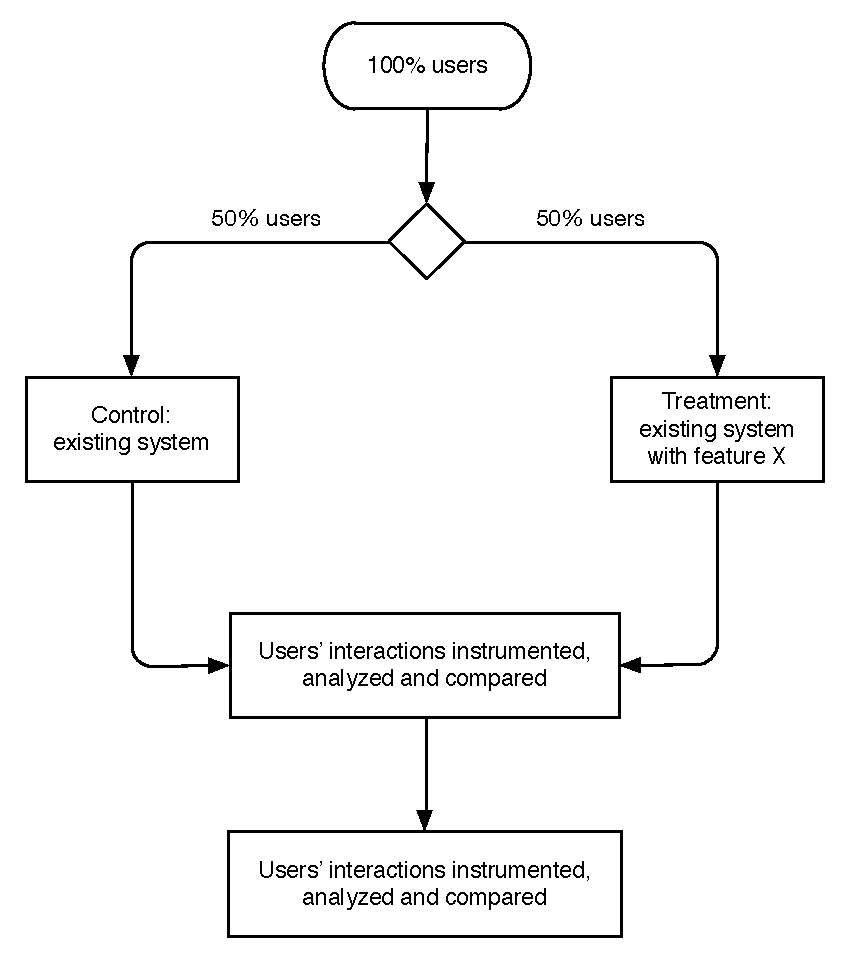
\includegraphics[width=0.7\textwidth]{Figures/ab-test-flow}
    \caption{The flow of an A/B test.}
    \label{fig:ab_flow}
\end{figure}

One word in the previous paragraph, ``randomly'', warrants some discussion. To be able to establish a causal relationship between the selected variant and the evaluation, the variant selection must indeed be completely random, and not based on what Kohavi et al. term ``any old which way''~\cite{Kohavi2007}.

This point \emph{must} be kept in mind when designing adaptive systems based on controlled experiments, as in our case.

\subsection{Running a feature experiment}
\label{approach:running_feature_experiment}

Ideally at this point, we have identified several significant clusters of users. Next we want to find viable ways of adapting the product to better suit each user.

Given a set of candidate product alterations $A$, we want to give each user the combination of these that maximizes some performance measure $P$. However, we have no predictive bias to start us off on solving this.

The approach taken in this implementation is a simple one, which relies on conducting a single A/B test up front for each proposed product alteration. An important part of this phase is to log each selected variant with the \emph{same person identifier} as is used for other event instrumentation, as discussed in section~\ref{approach:sub:generating_data}.

% This approach enables us to see up-front whether there are any significant variances in feature adoption between the clusters. If there are, we can adapt the service by selecting the more successful variation of the feature for all users in the relevant clusters. If not, we have a feature that affects all users equally -- at least with regard to cluster granularity.

\subsection{Evaluation metrics} % (fold)
\label{approach:sec:evaluation_metrics}

When considering which variation of a product feature to prefer, we need to be able to measure their relative success rates. As introduced above, this involves determining an overall evaluation criterion -- an OEC.

As for any user-facing product, the main objective is achieving user happiness. However, user happiness is hard to objectively define. For a service like appear.in, though, activity level serves as an adequate indicator of user happiness, as unhappy users have more than enough alternative applications that could cater to their needs.

Simply put, we basically assume that the following hypothesis holds:

\begin{hypothesis}
  Happy users use the service more than unhappy users.
\end{hypothesis}

Furthermore, we seldom need a measure of \emph{user happiness} to determine the relative success of variations of a product feature. Some parts of the product have clearly defined goals themselves.

The perhaps most obvious example of this is the landing page, whose main objective is to get people to try out the product. We can define the performance of the landing page in terms of the percentage of users that continue on to try out the product.

\section{Adaptation component} % (fold)
\label{approach:sec:adaptation_component}

In the adaptation component, we want to select the variation which is most likely to provide the best experience for the user.

In other words, given a user $u$ in cluster $c$ and a set of variations $V$, we choose the variation that is more likely to maximize our selected objective function. That is,

\begin{equation}
  \text{preferred}(c, V) = \argmax_{v \in V} \text{score}(c, v)
\end{equation}

The scoring function will in our case simply be the ratio of cluster $c$ members who were ``converted'' during the experiment, ie. who achieved the designated goal, after having been presented with variation $v$.

\begin{equation}
  \text{score}_{c,v} = \frac{\text{converted}_{c,v}}{\text{participants}_{c,v}}
\end{equation}

Given a recent set of clusters and experiment results for the users within them, the adaptation component has what it needs to select a preferred variation based on this heuristic.

\subsection{Applying the personalized feature set} % (fold)
\label{approach:sec:applying_the_personalized_feature_set}

Since well before this project, appear.in had a way of toggling features based on external criteria. The existing model allowed for overriding various settings, as well as pre-releasing features internally, using URL parameters.

We call this scheme ``URL-based feature switching''. Some examples are listed in table~\ref{tab:feature_switches}.

\begin{table}[h]
  \centering
    \begin{tabular}{|l|l|}
      \hline
      Parameter setting    & Effect \\ \hline
      \texttt{?video=off}  & Turn off video by default. \\
      \texttt{?audio=off}  & Mute microphone by default. \\
      \texttt{?followRoom} & Turn on experimental ``follow room'' functionality. \\
      \hline
    \end{tabular}
  \caption{By appending feature switches to the room URL, various effects can be achieved.}
  \label{tab:feature_switches}
\end{table}

Enabling user adaptation thus became a simple matter of extending this model by allowing for feature values to be dictated by our adaptation component.

In the current codebase, the setting of each feature value happens like so:

\begin{minted}[gobble=2]{javascript}
  var features = {
      // ...
      isVideoDisabledByDefault: $routeParams.video === "off",
      isAudioDisabledByDefault: $routeParams.audio === "off"
  };
\end{minted}

Here, \verb|$routeParams| contains the parameters set in the URL, as described above. In the same way, we can perform an external call with the current user id to the adaptation component described above, and apply the desired feature set in a similar way.
